\chapter{Requisitos}

\section{Visão geral do sistema}
% nesta secção, apresentar o PRODUTO proposto: um sistema para apoiar projetos de I&D que incluem recolha de dados fisiológicos, que podem ocorrer em laboratório, como em ambulatório Identificar os atores envolvidos e as suas motivações 
O produto proposto é um sistema que permite a recolha de dados fisiológicos de pessoas e a respetiva revisão dos dados recolhidos por parte dos profissionais, responsáveis pelo estudo. A recolha pode ocorrer em laboratório ou em ambulatório, isto é, os participantes podem recolher estes dados presencialmente ou remotamente. Um dos objetivos deste sistema é apoiar projetos de \gls{ID} que são cada vez mais importantes para reduzir a incerteza na utilização de determinadas tecnologias e ideias.
\par 
O sistema irá ser composto por uma aplicação móvel que tem como objetivo principal recolher dados dos sensores, e uma aplicação Web para visualizar esses dados recolhidos. O dispositivo com sensores utilizado poderá ser o VitalJacket e os dados fisiológicos recolhidos poderão ser a frequência cardíaca, \gls{ECG} e acelerómetro. Poderá ser utilizado este dispositivo pois como já fez parte de outros estudos, é um equipamento válido e permite recolher os tipos de dados que pretendemos. O sistema irá contemplar então dois atores distintos:
\begin{itemize}
  \item Revisor/Investigador que tem como objetivo rever dados inseridos pelos diferentes utilizadores
  \item Participante(alvo de estudo) que tem como função recolher dados vitais e acelerómetro para posteriormente serem revistos pelo revisor/investigador
\end{itemize}
\newpage
\section{Casos de Utilização na Colheita de Dados}

Na figura \ref{f:usecaseandroidapp} podemos visualizar um diagrama com os casos de utilização (cenários-objetivo) da aplicação móvel. O principal ator desta aplicação é o participante(alvo de estudo) que tem que recolher várias sessões de leitura para serem posteriormente analisadas e visualizadas por Investigadores/Revisores.  Uma breve descrição de cada caso de utilização é apresentada na tabela \ref{t:and-usecase}.
\par
O ator é um participante de um estudo e pode ter sido selecionado pelos responsáveis de duas maneiras diferentes, eventualmente como voluntário ou como doente. 

\begin{figure}[H]
  \centering
  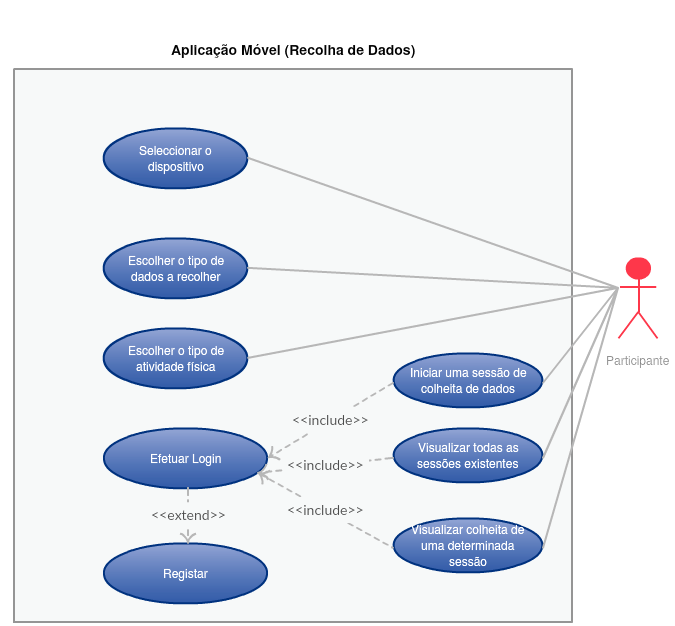
\includegraphics[width=0.8\textwidth]{imgs/app-and-usecase.png}
  \caption[Diagrama de casos de uso da aplicação móvel para colheita de dados]{Diagrama de casos de uso da aplicação móvel para colheita de dados}
  
  \label{f:usecaseandroidapp}
\end{figure}

\newpage


\begin{table}[H]
\centering
\label{t:and-usecase}
\begin{tabular}{|l|l|}
\rowcolor[HTML]{FFCE93} \hline
{\color[HTML]{000000} \textbf{Caso de utilização}} & {\color[HTML]{000000} \textbf{Propósito do caso de utilização}}  \\
\hline
Efetuar Login                                 & \begin{tabular}[c]{@{}l@{}}O Participante deve conseguir entrar com a sua conta na \\aplicação móvel.\end{tabular}   \\ \hline


Registar                                      & \begin{tabular}[c]{@{}l@{}} O Participante que vai participar no estudo pode criar uma \\nova  conta.\end{tabular} \\ \hline


\begin{tabular}[c]{@{}l@{}}Escolher o tipo de \\ atividade física \end{tabular}&\begin{tabular}[c]{@{}l@{}} Consoante o tipo de atividade física que estiver a efetuar, o \\participante pode escolher a mais adequada. \end{tabular}\\ \hline


\begin{tabular}[c]{@{}l@{}}Escolher o tipo de \\dados a recolher \end{tabular}          & \begin{tabular}[c]{@{}l@{}}Tem que existir a possibilidade de filtrar o tipo de dados que \\ são para ser recolhidos numa determinada colheita. Pode \\ocorrer a situação de recolher todos ao mesmo tempo.\end{tabular}  \\ \hline



Selecionar o dispositivo  & \begin{tabular}[c]{@{}l@{}}Para se conseguir efetuar a colheita dos dados um \\dispositivo válido tem que ser selecionado. \end{tabular}\\ \hline


\begin{tabular}[c]{@{}l@{}}Iniciar uma sessão \\de colheita de dados \end{tabular}       & Pode iniciar uma nova colheita de dados. \\ \hline


\begin{tabular}[c]{@{}l@{}}Visualizar todas as \\sessões existentes \end{tabular}        & \begin{tabular}[c]{@{}l@{}}O Participante pode visualizar todas as sessões em que \\recolheu dados. \end{tabular}\\ \hline


\begin{tabular}[c]{@{}l@{}}Visualizar colheita de \\ uma determinada sessão \end{tabular}&\begin{tabular}[c]{@{}l@{}} O Participante ao escolher uma colheita das várias\\ apresentadas pode visualizar ao detalhe todos os dados \\recolhidos numa determinada sessão.\end{tabular} \\ \hline                        
\end{tabular}
\caption{Breve descrição dos casos de utilização da aplicação de colheita de dados}
\end{table}

\section{Casos de Utilização na Revisão de Dados}

Na figura \ref{f:usecasewebapp} podemos visualizar todos os casos de uso (cenários-objetivo) da aplicação web. O principal ator desta aplicação é o revisor/investigador que pode fazer uma revisão das várias sessões de recolha efetuadas pelos participantes. Uma breve descrição de cada caso de utilização é apresentada na tabela \ref{t:web-usecase}

\begin{figure}[H]
  \centering
  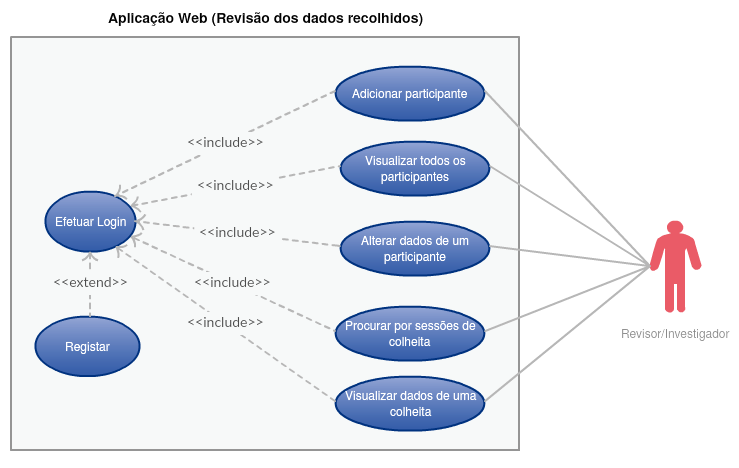
\includegraphics[width=0.8\textwidth]{imgs/app-web-usecase.png}
  \caption[Diagrama de casos de uso da aplicação web]{Diagrama de casos de uso da aplicação web}
  
  \label{f:usecasewebapp}
\end{figure}



\begin{table}[H]
\centering
\label{t:web-usecase}
\begin{tabular}{|l|l|}
\rowcolor[HTML]{FFCE93} \hline
{\color[HTML]{000000} \textbf{Caso de utilização}} & {\color[HTML]{000000} \textbf{Propósito do caso de utilização}}  \\
\hline
Efetuar Login                                 & \begin{tabular}[c]{@{}l@{}}O Revisor deve conseguir entrar com a sua conta na \\aplicação web.\end{tabular}   \\ \hline


Registar                                      & \begin{tabular}[c]{@{}l@{}} O Revisor pode criar uma nova  conta.\end{tabular} \\ \hline


\begin{tabular}[c]{@{}l@{}}Adicionar participante \end{tabular}&\begin{tabular}[c]{@{}l@{}} O Revisor deve poder adicionar um novo participante \\como seu alvo de estudo.\end{tabular}\\ \hline


\begin{tabular}[c]{@{}l@{}}Visualizar todos \\os participantes \end{tabular}   & \begin{tabular}[c]{@{}l@{}} O Revisor deve conseguir visualizar todos os \\ participantes do seu alvo de estudo.\end{tabular}  \\ \hline



\begin{tabular}[c]{@{}l@{}}Alterar dados \\de um participante \end{tabular}   & \begin{tabular}[c]{@{}l@{}} A edição dos dados demográficos do participante deve \\ser possível.\end{tabular}\\ \hline


\begin{tabular}[c]{@{}l@{}}Iniciar uma sessão \\de colheita de dados \end{tabular}       & Pode iniciar uma nova colheita de dados. \\ \hline


\begin{tabular}[c]{@{}l@{}}Procurar por \\sessões de colheita \end{tabular}        & \begin{tabular}[c]{@{}l@{}}Relativamente a um participante deve ser possível  pesquisar \\colheitas efetuadas num determinado intervalo de tempo. \end{tabular}\\ \hline


\begin{tabular}[c]{@{}l@{}}Visualizar dados de \\ uma determinada sessão \\de colheita \end{tabular}&\begin{tabular}[c]{@{}l@{}} O Revisor depois de pesquisar as sessões para um determinado \\intervalo, deve poder ver os dados recolhidos para cada uma \\das sesões\end{tabular} \\ \hline                        
\end{tabular}
\caption{Breve descrição dos casos de utilização da aplicação de Revisão}
\end{table}

\cleardoublepage